The digital components layer will consist of 4 devices. The first is a Raspberry
PI. This will act as the main computer of the system. It will the major hub for
the data both from the server: the UI, and the micro controllers. The other 3
components will all be ESP32 micro controllers, but they will each serve a
different purpose. An ESP32 will receive information from a thermometer sensor
and relay it to the heat control ESP32. Based on what the temperature is, the
heat control ESP32 will trigger the relay to activate or deactivate the heating
element. The final ESP32 will be used to trigger the relay to turn on the pump
based on what the message broker instructs it to do.   

\begin{figure}[h!]
	\centering
 	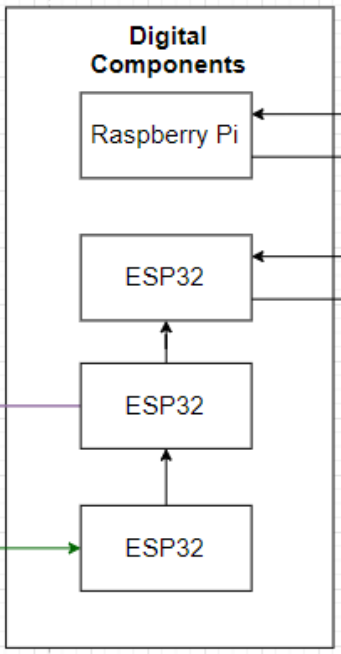
\includegraphics[width=0.30\textwidth]{images/digital_components.png}
  \caption{Digital Components Subsystem Description Diagram}
\end{figure}

\subsection{Raspberry PI Subsystem}
The Raspberry PI will host the web server and the MQTT client. The Raspberry PI will
receive information from the web server about what the user inputted via the UI.
It will then take that information and relay it to the micro controllers using
the MQTT protocol. The Raspberry PI will then receive sensor data from the
micro controllers through MQTT protocol and send the information in the web
server for storing. 

\subsubsection{Assumptions}
The Raspberry PI will have a power supply. It will remain safe from the elements. It
will be connected to the network. It will have unbroken communication with the
web server. It will communicate with the micro controllers through the MQTT protocol.

\subsubsection{Responsibilities}
It will receive data from the web server to determine how to operate the pump.
It will instruct the micro-controller to activate or deactivate based on the
information it receives. It will relay sensor information to the web server so
that it can be displayed.

\subsubsection{Subsystem Interfaces}
\begin {table}[H]
  \caption {Raspberry Pi Subsystem interfaces} 
  \begin{center}
    \begin{tabular}{ | p{5cm} | p{4cm} | p{4cm} |}
      \hline
      Description & Inputs & Outputs \\ \hline
      Web Service API & \pbox{4cm}{Information from UI input by user} & \pbox{4cm}{Sensor Data and status}  \\ \hline
      ESP32 & \pbox{4cm}{Sensor data from ESP32} & \pbox{4cm}{Messages instructing microcontrollers what to do}  \\ \hline
    \end{tabular}
  \end{center}
\end{table}

\subsection{Thermometer Sensor Subsytem}
This micro-controller will monitor data from the thermometer sensor. It will then
relay that information back to the message broker. 

\subsubsection{Assumptions}
The microcontroller will have a power supply. It will remain safe from the elements. It
will be connected to the network. It will be connected to the thermometer
sensor. It will operate through MQTT protocol.

\subsubsection{Responsibilities}
It will monitor the data from the thermometer sensor and relay that information
using the MQTT protocol. 

\subsubsection{Subsystem Interfaces}
\begin {table}[H]
  \caption {Thermometer Sensor Subsystem interfaces} 
  \begin{center}
    \begin{tabular}{ | p{5cm} | p{4cm} | p{4cm} |}
      \hline
      Description & Inputs & Outputs \\ \hline
      Thermometer Sensor & \pbox{4cm}{Data from thermometer sensor} & \pbox{4cm}{message to communicate sensor data}  \\ \hline
    \end{tabular}
  \end{center}
\end{table}

\subsection{Heat Control Subsystem}
The microcontroller will await messages from the message broker. The message
broker will receive information from the thermometer ESP32. If the temperature
is too low, the message broker will send a message to this microcontroller to
trigger the relay and allow power to flow to the heating element. If the
temperature gets too high on the heating element, the message broker will tell
this microcontroller to deactivate the heating element.

\subsubsection{Assumptions}
The microcontroller will have a power supply. It will remain safe from the elements. It
will be connected to the network. It will be connected to the relay that
controls power to the heating element. It will operate through MQTT protocol.

\subsubsection{Responsibilities}
It will activate or deactivate the relay that controls the power flow to the
heating element based on what the message broker instructs it to do. It will
send a status message back to the message broker. 

\subsubsection{Subsystem Interfaces}
\begin {table}[H]
  \caption {Heat Control Subsystem interfaces} 
  \begin{center}
    \begin{tabular}{ | p{5cm} | p{4cm} | p{4cm} |}
      \hline
      Description & Inputs & Outputs \\ \hline
      Heating Element Relay & \pbox{4cm}{message from RBP} & \pbox{4cm}{relay trigger and status message}  \\ \hline
    \end{tabular}
  \end{center}
\end{table}

\subsection{Pump Control Subsystem}
This microcontroller will await messages from the message broker. When the
message broker sends it the message to turn on the pump, the microcontroller
will trigger the relay to allow power to go to the pump. When the message broker
sends the message to turn off the pump, the microcontroller will cease sending
power to the relay, causing it to close, and power will not be supplied to the
pump.

\subsubsection{Assumptions}
The microcontroller will have a power supply. It will remain safe from the elements. It
will be connected to the network. It will be connected to the pump relay. It will operate through MQTT protocol.

\subsubsection{Responsibilities}
It will trigger the relay that will supply power to the pump based on the
message it receives from the message broker. It will then return a status
message to the message broker.

\subsubsection{Subsystem Interfaces}

\begin {table}[H]
\caption {Pump Control Subsystem interfaces} 
\begin{center}
    \begin{tabular}{ | p{6cm} | p{3cm} | p{3cm} |}
    \hline
    Description & Inputs & Outputs \\ \hline
    Pump Relay & \pbox{3cm}{message from RBP} & \pbox{3cm}{relay trigger and status message}  \\ \hline
    \end{tabular}
\end{center}
\end{table}
